\chapter{全景漫游行业的市场现状}

\section{全景漫游技术总览}

全景漫游是由多种技术组合而成,其核心目的都是服务于将全景场景呈现给用户体验的过程。它是计算机仿真技术的重要方向之一,是计算机图形仿真模拟、多媒体传感交互及网络通信等多种技术的综合,是一门富有挑战性的前沿交叉技术应用学科,具有广阔的研究领域。根据不同阶段所应用的技术类别,可以得出全景漫游的技术路径图,如图\ref{fig:process}所示,最左为真实场景,最右为用户,技术所起到的作用就是将场景与用户连接起来。

\begin{figure}[htp]
\centering
\fbox{
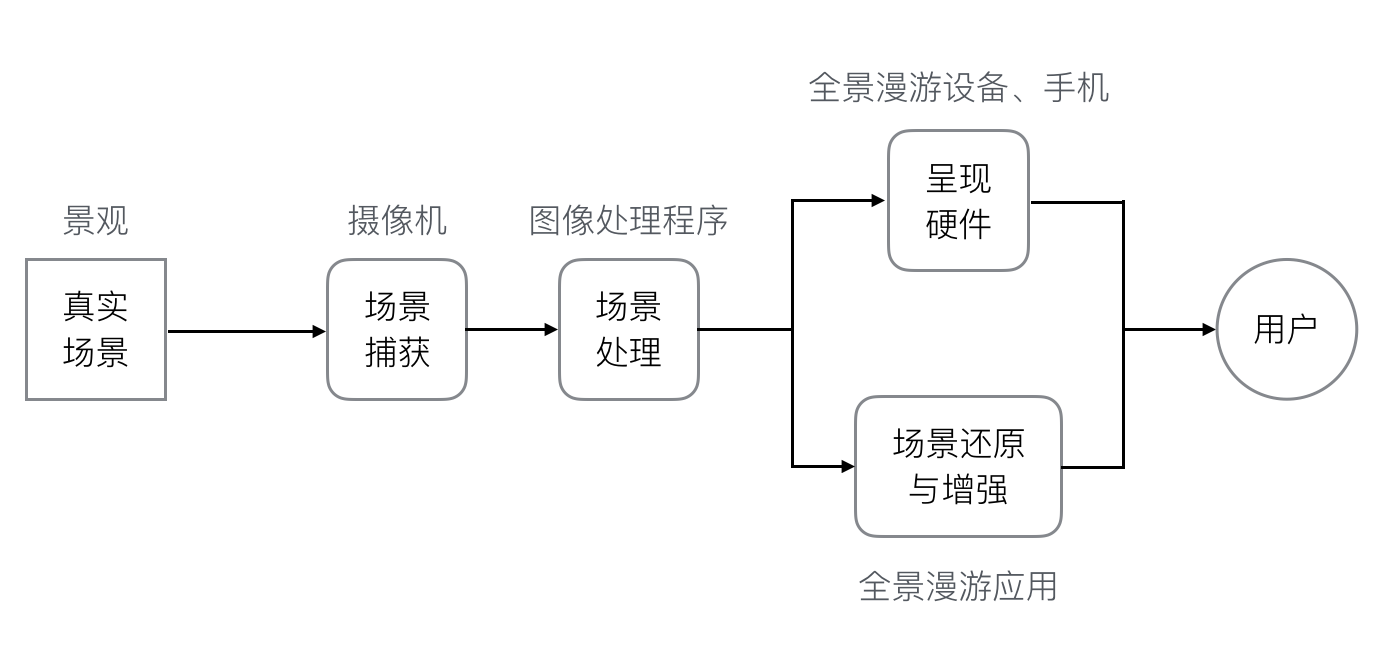
\includegraphics[width=.7\textwidth]{process}
}
\caption{全景漫游的技术路径}
\label{fig:process}
\end{figure}

全景漫游技术按载体分类可分为:
\begin{description}
\item[场景捕获硬件技术]视频捕获设备及其保障设备,用以采集全景漫游的视频、图片、音频等素材。
\item[场景呈现硬件技术] 主要包括 VR 眼镜、VR 互动手柄、VR 主机等。
\item[场景处理技术] 场景规划设计、场景素材的保存与传输以及相应程序开发等。
\item[场景还原与增强技术] 将场景素材与功能模块有机地整合,提供给用户身临其境般的全景漫游体验。
\end{description}

\subsection{场景呈现硬件技术}
相对而言,硬件技术相比于后两者进入门槛更高。目前市场上三大 VR 硬件厂商 OculusRift、HTCVive 和 PlayStationVR 几乎垄断了高端 VR 播放设备市场。之后加入 VR 市场的企业(如暴风、大朋、3Glasses、蚁视等)几乎都放低了姿态,推出了价格低廉但基本满足播放功能的入门级 VR 眼镜作为卖点。但随着 Google Cardboard 的推出,这款几乎没有成本可言的开源“硬件”迅速占领了低端 VR 硬件行业相当客观的市场份额。

\subsection{场景捕获硬件技术}
场景捕获技术的难点在于实时捕获,合成全景照片是一般手机都拥有的功能,大致原理就是捕获数张连续且相近的照片并通过算法进行合成球形场景。但实时场景捕获硬件的成本因其同步的特性更为高昂,目前市面上已有的厂商例如 Google JUMP、NOKIA OZO 等均是将现有平面镜头进行堆叠排布并通过后期处理合成虚拟场景,且这种方式因需要较多的镜头来堆砌同时刻的画面所以硬件成本非常高。目前市面上尚只有堆叠摄像头这一种方式进行全景场景捕获,而光场摄影等技术仍处在技术攻关阶段,相信不远的将来有可能出现消费级的场景捕获硬件。

\subsection{场景处理技术}
场景处理是目前全景漫游软件领域需要重点攻克的最大难关,但市面上各企业已基本做到自给自足的技术支持。全景漫游所依赖的基础是图像信号的捕获、加工与储存,而这些方面已有较多成功经验。目前 Web 端视频播放协议有以下两种:Real Time Messaging Protocol(实时消息传输协议,简称 RTMP)和 HTTP Live Streaming(HTTP 渐进下载,简称 HLS)。这两者是孑然不同的两种协议,而且 iPhone 等手机由于不自带支持 Flash 播放,一般考虑全端支持的流媒体播放会选用 HLS 作为传输协议,即对视频做切片,边播放边加载下一时段的切片。

\subsection{场景还原与增强技术}
场景还原与增强是与用户直接相连的部分,可以说前面的技术都是起为其保驾护航的功能。其中场景还原部分为计算机图形学的范畴,例如图像在空间上的曲率计算等,主要涉及到的技术有 OpenGL/WebGL 等,用于将二维图像还原成球状的场景。而场景增强技术则是本文所讨论的重点,其主要功能是为还原出的场景增添互动性,以使得用户可以自如地进行漫游体验。场景处理技术以软件形式作为载体,根据运行平台不同可分为直接编译代码至设备端的三维引擎软件和利用网页技术进行场景构建并可以运行于任意浏览器的 web 框架两种,以下以三款目前较为热门的软件框架进行介绍:

\paragraph{三维引擎软件:Unity 3D}

Unity 3D 是由 Unity Technologies 开发的一个使用脚本和即时编辑工具可视化创建例如三维场景、数字建筑体、实时三维动画等多类型互动内容的跨平台综合型游戏开发工具。\endnote{百度百科.Unity 3D-百度百科. http://t.cn/RJDzA1F[EB]}

\paragraph{Web 全景漫游框架:Krpano}
Krpano 是一个用来呈现各种全景图像和交互式虚拟全景场景的查看器。可作为 Flash 或 HTML5 应用程序在 Web 上使用。并附有利用拖拽全景生成场景的 Krpano Tools 以供开发者快速生成用以展示的全景场景。本文将应用其进行部分设计案例的制作与演示。

\paragraph{Web 全景漫游框架:A-Frame}
A-Frame 是一个用 Web 技术构建虚拟现实体验的框架。使用超文本标记语言及实体组件来构建场景,可应用于普通网页及一般移动网页页面,方便地传输到其他多种设备端。本文将应用其进行部分设计案例的制作与演示。

\section{全景漫游市场前景}

2016 年,伴随着三大虚拟现实设备的出售,未来 2-3 年的时间内虚拟现实设备的市场普及率将快速提升。2020 年时,虚拟现实生态圈初步形成,内容、服务等盈利模式将逐步成熟,全球虚拟市场规模将达到 404 亿美元,其中虚拟现实的游戏市场规模或可高达 149.5 亿美元。\endnote{VRZINC. 易观智库:2020年全球VR市场规模将达到404亿美元. \newline http://vreyes.baijia.baidu.com/article/595977[EB]}

虚拟现实(VR/AR)产业市场具有良好前景,2015 年中国虚拟现实行业市场规模为 15.4 亿元人民币。显示设备融资占据首要地位,2015 年融资案例数量占比 30\%,融资额占比 69\%;内容制作的融资案例数量虽然占比 22\%,但融资额仅占比 6\%\endnote{赛迪智库.未来五年虚拟现实市场规模及前景展望. \newline http://www.elecfans.com/vr/444138.html[EB]}。可见虚拟现实及全景漫游方向的内容制作生产领域仍处于起步阶段,与硬件厂商等差距较大,但同时其中也孕育了巨大的商机。

虚拟内容开发受到消费者的热烈追捧,线下体验馆在各大商场增长迅速。由于中国虚拟现实市场主流设备仍以移动端虚拟眼镜为主,虚拟现实视频内容的开发难度低(不包换硬件设备),成本要远低于游戏内容,故当前市面上虚拟现实数字产品主要以视频为主。虚拟现实平台上已有约 2700 款视频和 800 款游戏。预计 2020 年中国虚拟现实设备出货量 820 万台,用户量将超过 2500 万人,见图\ref{fig:market}。

\begin{figure}[htp]
\centering
\fbox{
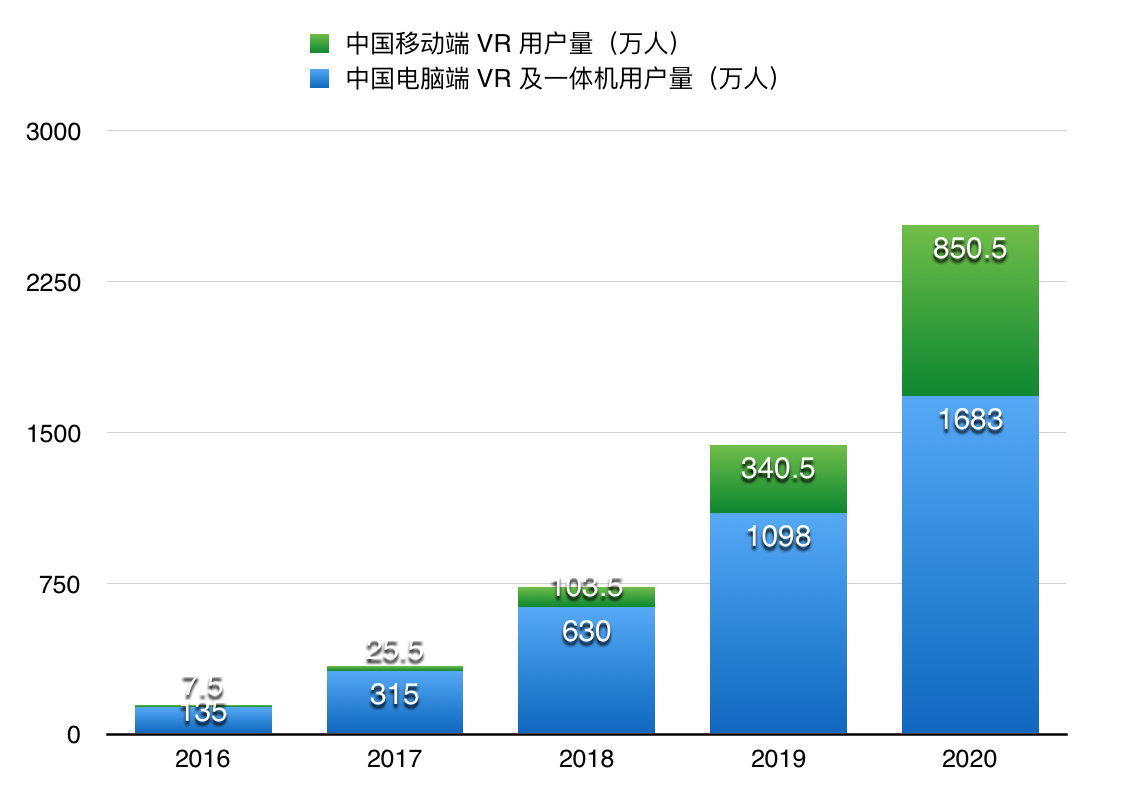
\includegraphics[width=.6\textwidth]{market}
}
\caption{2016-2020 年中国 VR 用户规模}
\label{fig:market}
\end{figure}

\section{全景漫游产业类别}
全景漫游产业按出发点可大体分为两类:
\begin{itemize}
	\item 以视频、游戏为主的虚拟内容提供商/平台商
	\item 涉及电商、教育、医疗、建筑等传统行业的行业融合应用服务商
\end{itemize}

短期而言,市场上比较活跃的是虚拟内容提供商,但长远而言,ToB 模式更利于产生更为健壮的全景漫游服务体系,对于高质内容的生产、分发和变现的模式也偏向于有传统大规模企业的行业服务商。

\section{全景漫游在工业领域的应用分析}
\subsection{复杂危险作业场景模拟及训练}

早在 20 世纪末,人们就已经认识到虚拟现实技术在仿真训练中的巨大作用。一篇 2001 年关于南非煤矿环境中利用虚拟现实进行安全训练的文章\endnote{Squelch A P. Virtual reality for mine safety training in South Africa[J]. Journal- South African Institute of Mining and Metallurgy, 2001, 101(4):209-216.}指出利用虚拟现实技术在特殊环境下进行安全训练的速度和可接受程度均高于使用传统图文或视频资料的对照组,说明了漫游行为在用户认知复杂环境中起到了不可或缺的作用。图\ref{fig:mine}即演示了一种突如其来的岩石垮塌的情形,需要被训练的工人根据情形作出操作来避免危险。

\begin{figure}[htp]
\centering
\fbox{
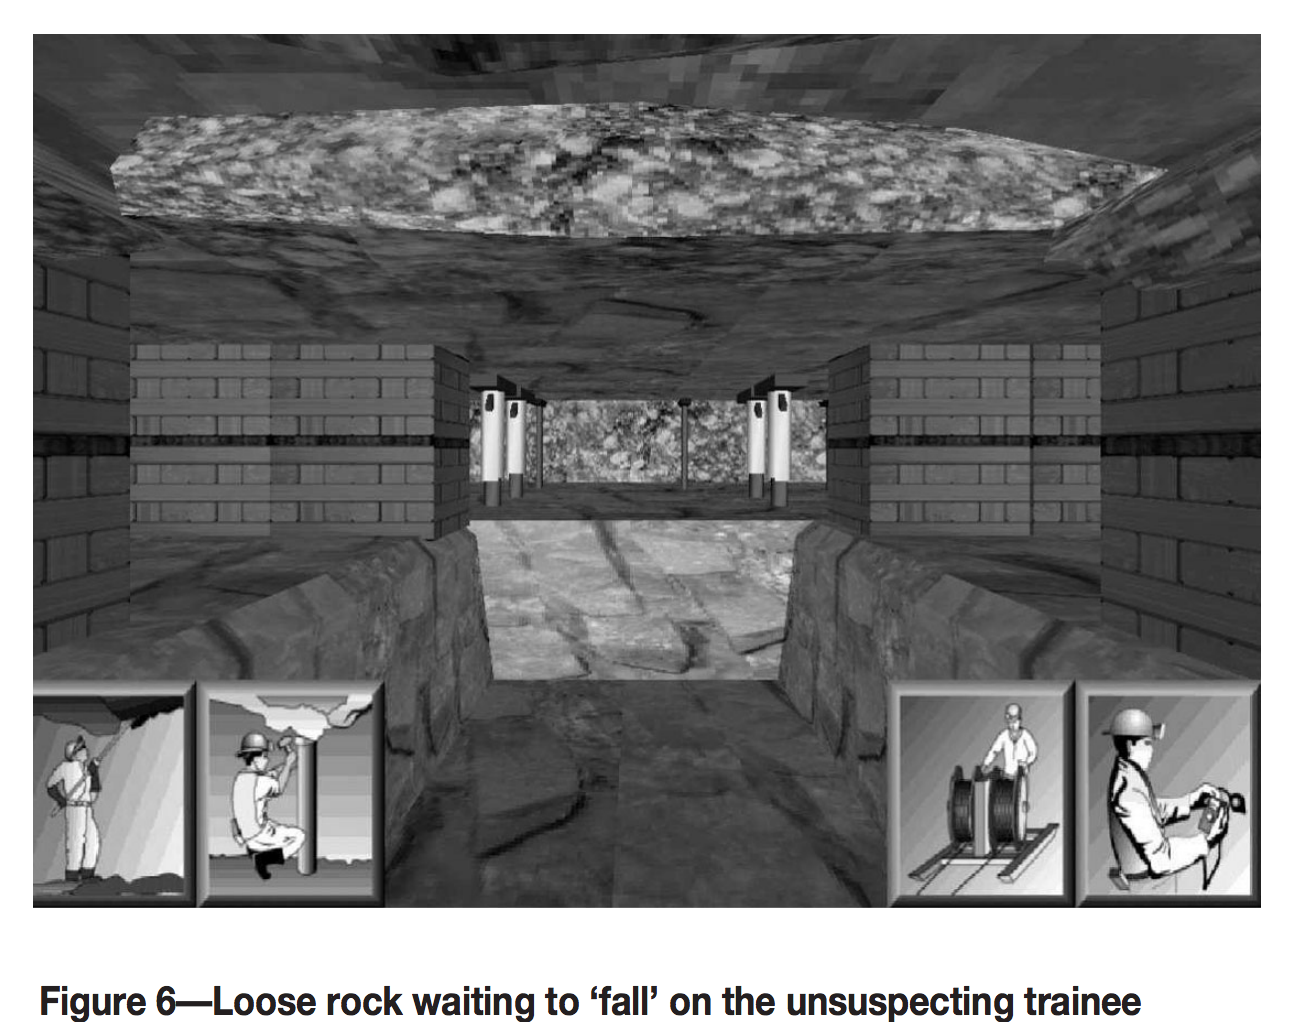
\includegraphics[width=.7\textwidth]{mine}
}
\caption{煤矿岩石垮塌模拟}
\label{fig:mine}
\end{figure}

虚拟现实技术还可被应用于航空航天训练、危险环境救援演练及其他人类无法安全、便捷进入的自然环境中,有效地拉近了使用者与模拟的真实环境间的认知距离,在保证安全的前提下高效完成训练任务。

\subsection{仿真虚拟环境}

另一种虚拟现实所应用的领域为建筑规划设计行业,因其所涉及的事物过于庞大,难以从普通的二维视图中体会其中的空间感,通过虚拟现实的技术则可以不必耗费大量精力搭建实物模型便能够身临其境般地感受建筑的尺度。

来自日本横滨国立大学教育学院的团队通过云计算 VR 系统帮助研究者快速搭建城市场景并实时查看、分享、交流与评估
\endnote{Zhang, Y., Shen, Z., Wang, K., Kobayashi, F., Lin, X. Cloud-based Virtual
Reality Integrated Automatic Presentation Script for Understanding Urban Design
Concepts in the Consensus Process: A Case Study of One Foundation Disaster Prevention
Park in China[J]. International Review for Spatial Planning and Sustainable Development,
5(1), 29-44. 2017.}。通过数字城市系统(如图\ref{fig:urban}),用户可以以自己想要的方式自主漫游整个场景。

\begin{figure}[htp]
\centering
\fbox{
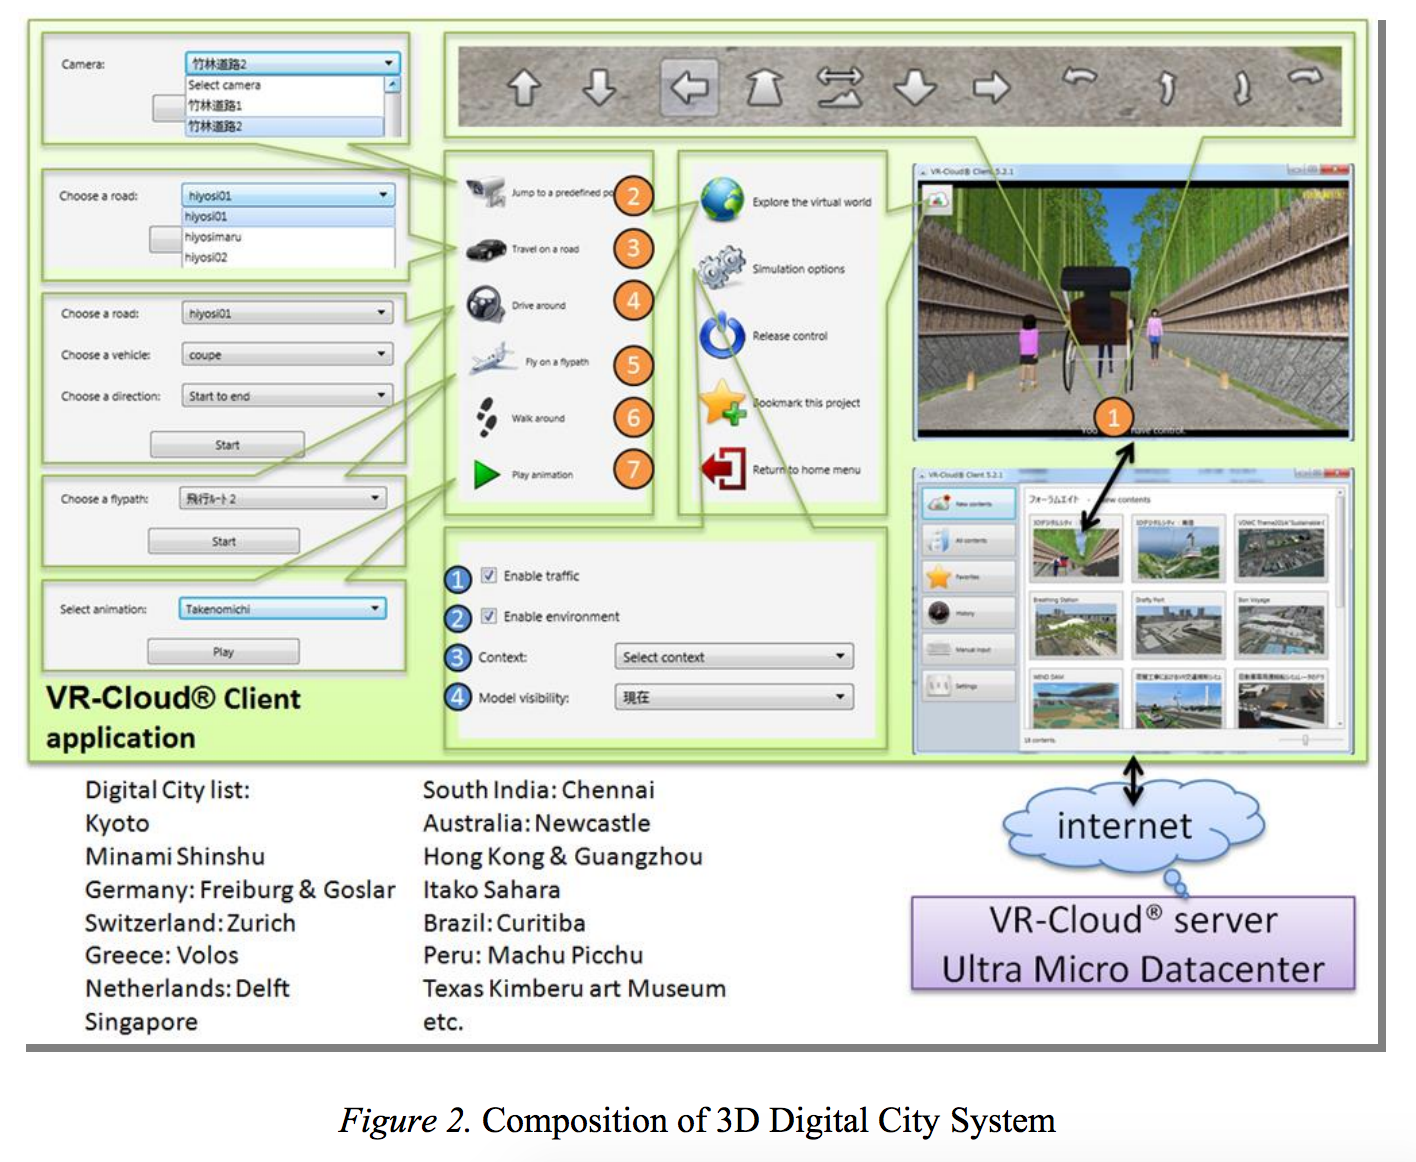
\includegraphics[width=.7\textwidth]{urban}
}
\caption{3D 数字城市系统}
\label{fig:urban}
\end{figure}

建筑信息模型(即 BIM)早已进入建筑工程项目的各个领域,全景漫游在技术和数据上几无障碍,且国内 BIM 技术也已较为成熟,充分利用全景漫游技术于建筑设计施工的方方面面将有利于设计者更直接地面对设计产物,提前发现设计中不完善的地方并加以改进。同时,将全景漫游的体验带给普通消费者,也有助于潜在购买者产生购买的欲望和动机。

\subsection{医疗康复}

医疗领域中虚拟现实技术的应用前景非常巨大,例如帮助因意外事故失去肢体或瘫痪的患者掌握使用假肢等。这些病患们的神经系统可以通过虚拟现实体验获得增强,他们能够在虚拟的环境内通过想象自己使用肢体进行运动、借由脑电波通过神经电位向计算机传递信号以操控虚拟环境内的肢体,在不断的反馈式训练过程中阶段性地磨合人与机器的灵敏程度,最终实现康复(见图\ref{fig:health})。相关专家称瘫痪的患者其实尚存在一些完好无损的神经组织,但因皮质和肌肉均未发射神经信号,这些神经将保持沉默数年。而利用虚拟现实的治疗将通过人机界面的训练重新唤醒这些神经,经过强化后将能够部分或完全地将大脑皮质运动区的信息传递到骨髓神经。

\begin{figure}[htp]
\centering
\fbox{
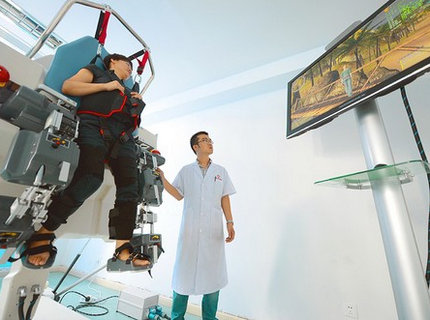
\includegraphics[width=.7\textwidth]{health}
}
\caption{瘫痪患者在进行治疗}
\label{fig:health}
\end{figure}

同时也有相关团队期望利用虚拟现实技术对患有自闭症的儿童进行适应性训练,在对超过 100 名智力正常的学龄儿童进行四面全沉浸式 CAVE VR 训练实验后,被试儿童们在情绪认知、情感表达及社交等领域表现出了显著的提升\endnote{Ip H H S, Wong S W L, Chan D F Y, et al. Virtual Reality Enabled Training for Social Adaptation in Inclusive Education Settings for School-Aged Children with Autism Spectrum Disorder (ASD)[M]// Blended Learning: Aligning Theory with Practices. Springer International Publishing, 2016.}。


\section{全景漫游现有移动应用分析}
\subsection{Ascape}

Ascape 这款美国公司开发的应用于 2017 年发布,主攻虚拟旅游市场。你能够通过 360° 无缝的全景视频身临其境般地切身体验视频中呈现的著名景点或人文古迹,探索只有历经千难万险才能体会的绮丽风光。伴随着你的移动,场景中镜头也会随之改变整个画面的位置和显示的角度,见图\ref{fig:ascape1}。

\begin{figure}[htp]
\centering
\fbox{
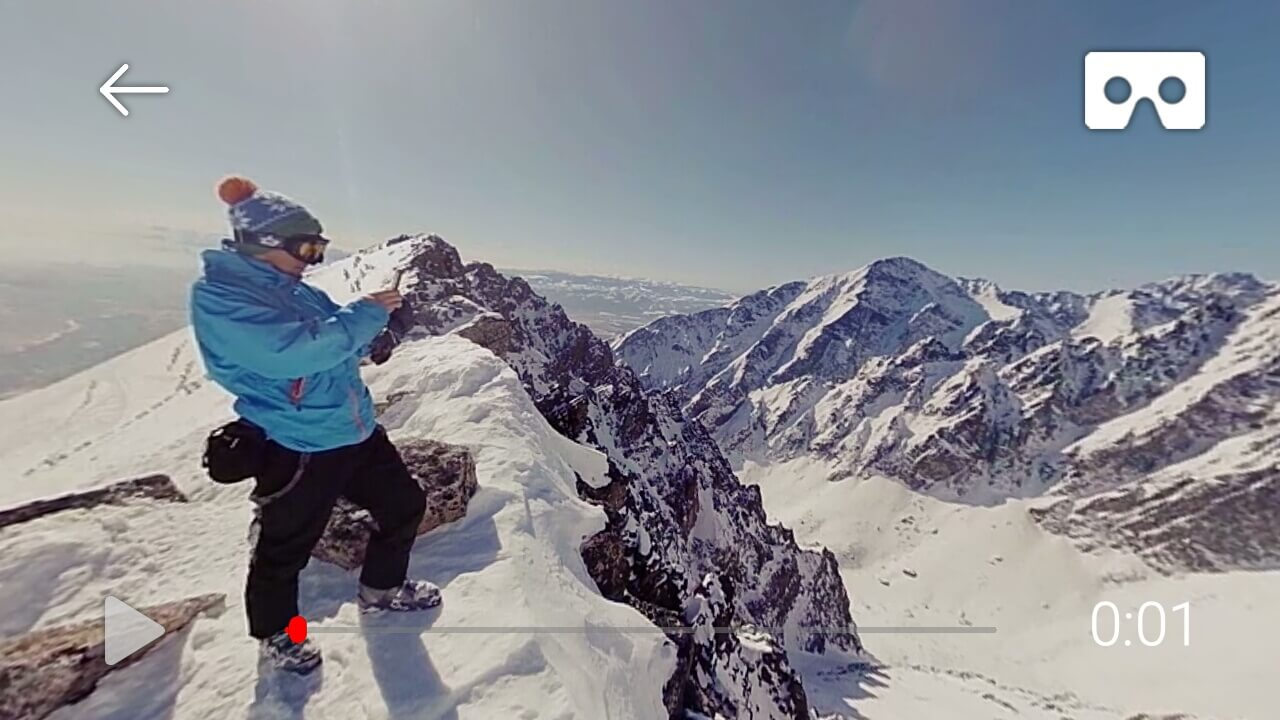
\includegraphics[width=.7\textwidth]{ascape2}
}
\caption{简洁的全景视频播放}
\label{fig:ascape1}
\end{figure}

同时,这款应用在移动应用传统界面上也继承了欧美一向以来的简约风格:“探索”页面采用卡片设计模式直观展示了新奇的场景;“发现”页面通过地图和名单两种模式展示了全球各地的场景选项;“我的旅行”也通过卡片模式展示了已下载的全景场景,见图\ref{fig:ascape2}。

\begin{figure}[htp]
\centering
\fbox{
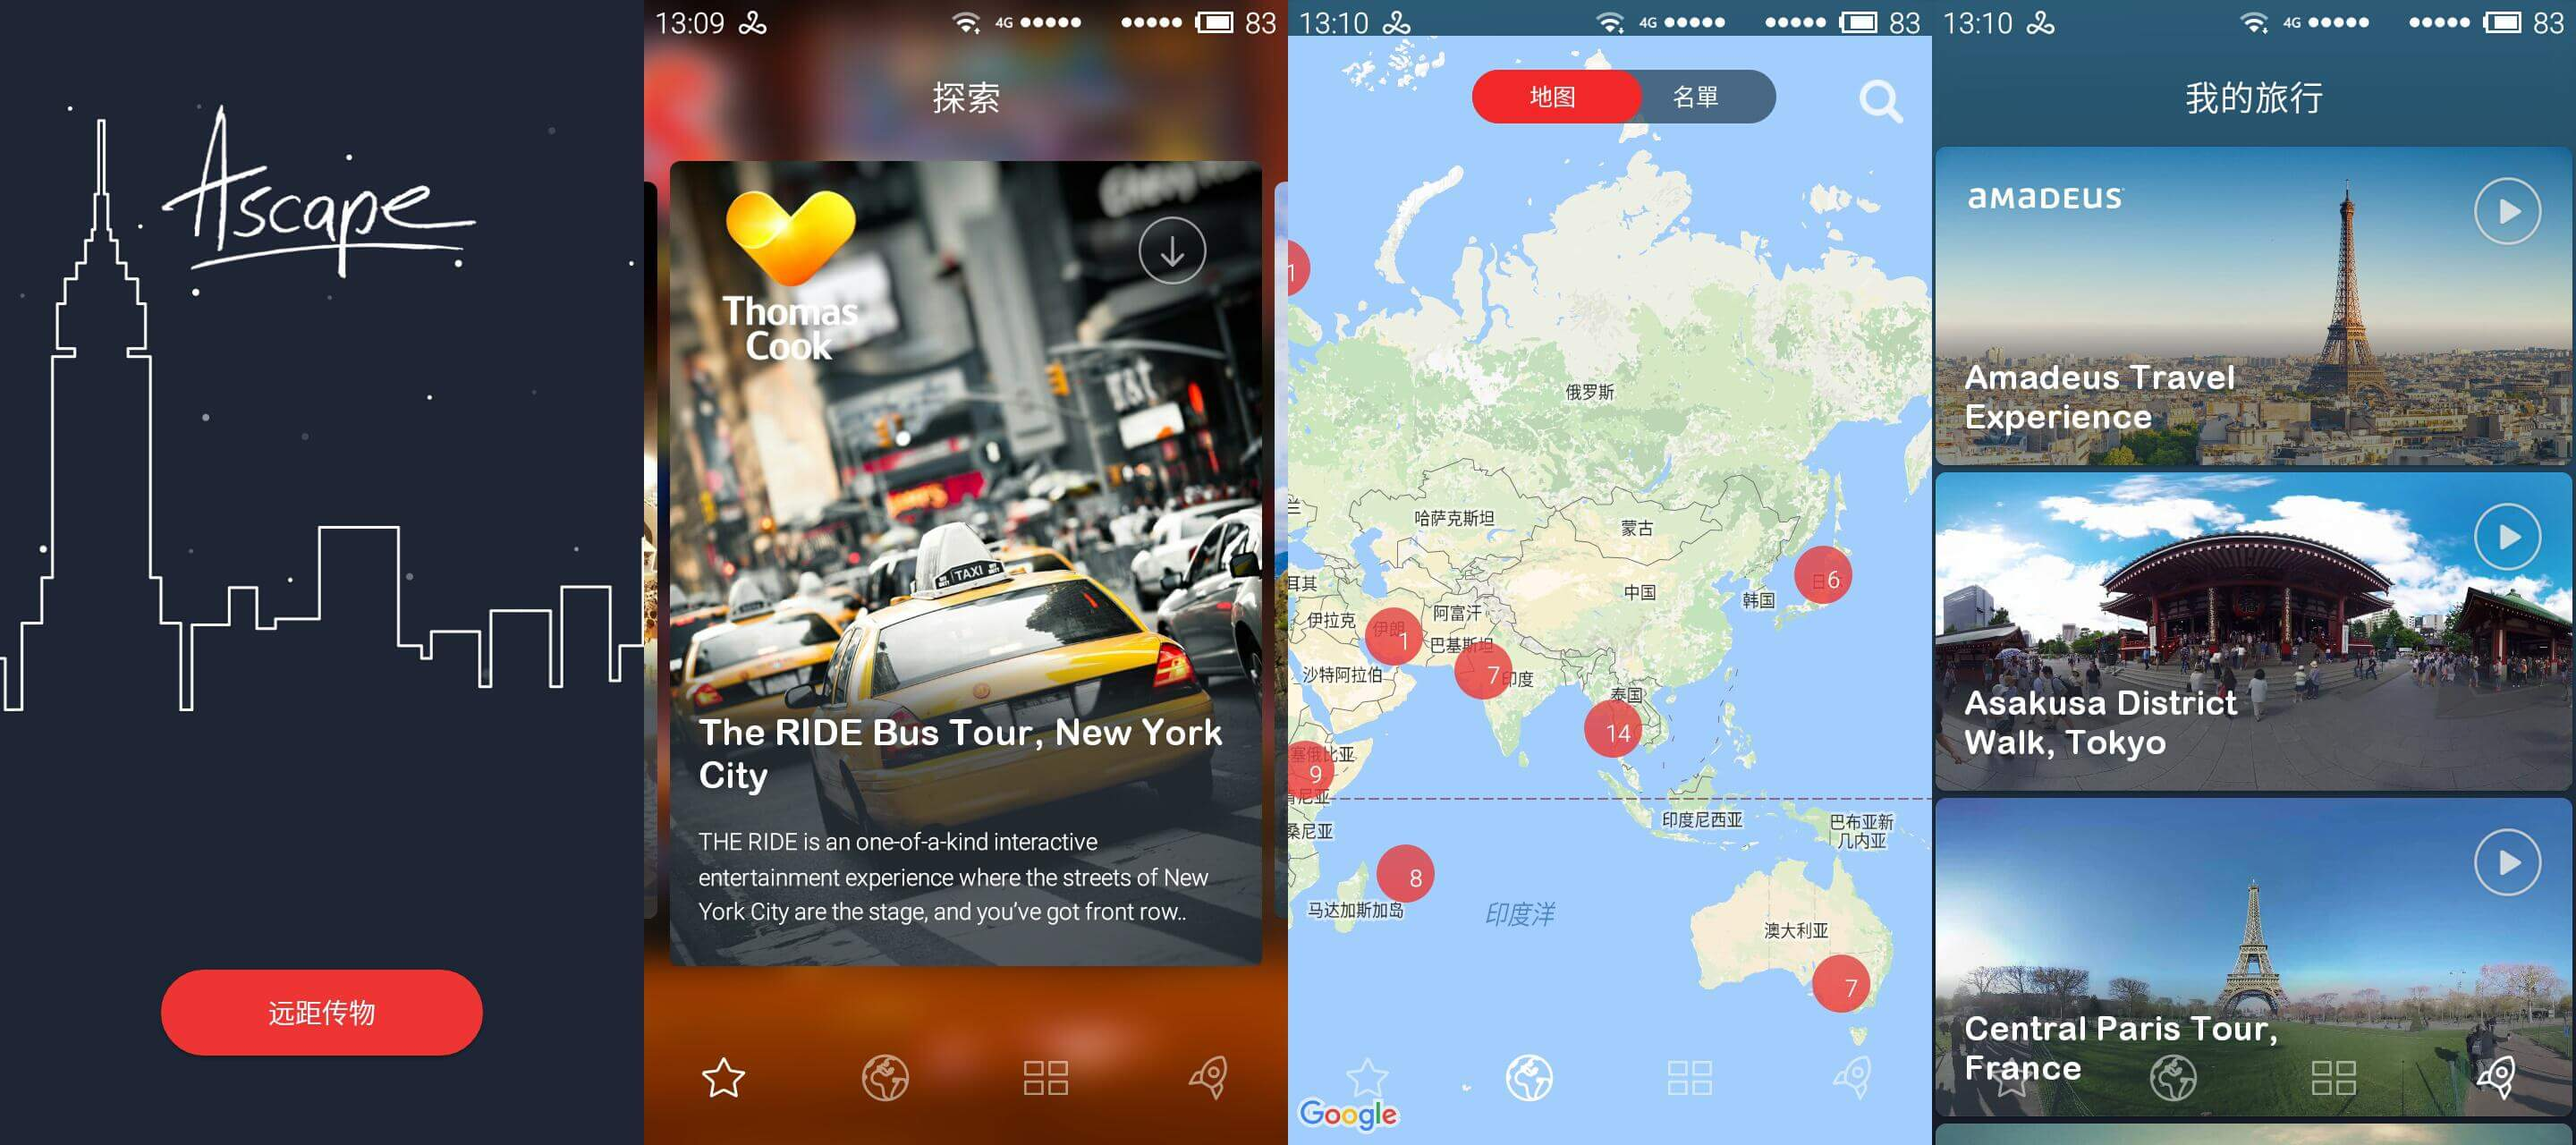
\includegraphics[width=.7\textwidth]{ascape1}
}
\caption{简洁的全景视频播放}
\label{fig:ascape2}
\end{figure}

\subsection{Fulldive}

Fulldive 这款美国公司开发的应用于 2016 年发布,是一个智能手机与虚拟场景连接的平台,进入应用后即进入了一个全景漫游的世界。场景内包含常用的网络视频、本地视频/图片、VR 相机、VR 浏览器等应用,同时支持从其内部市场下载更多基于其开发的虚拟现实应用,见图\ref{fig:fulldive1}。

\begin{figure}[htp]
\centering
\fbox{
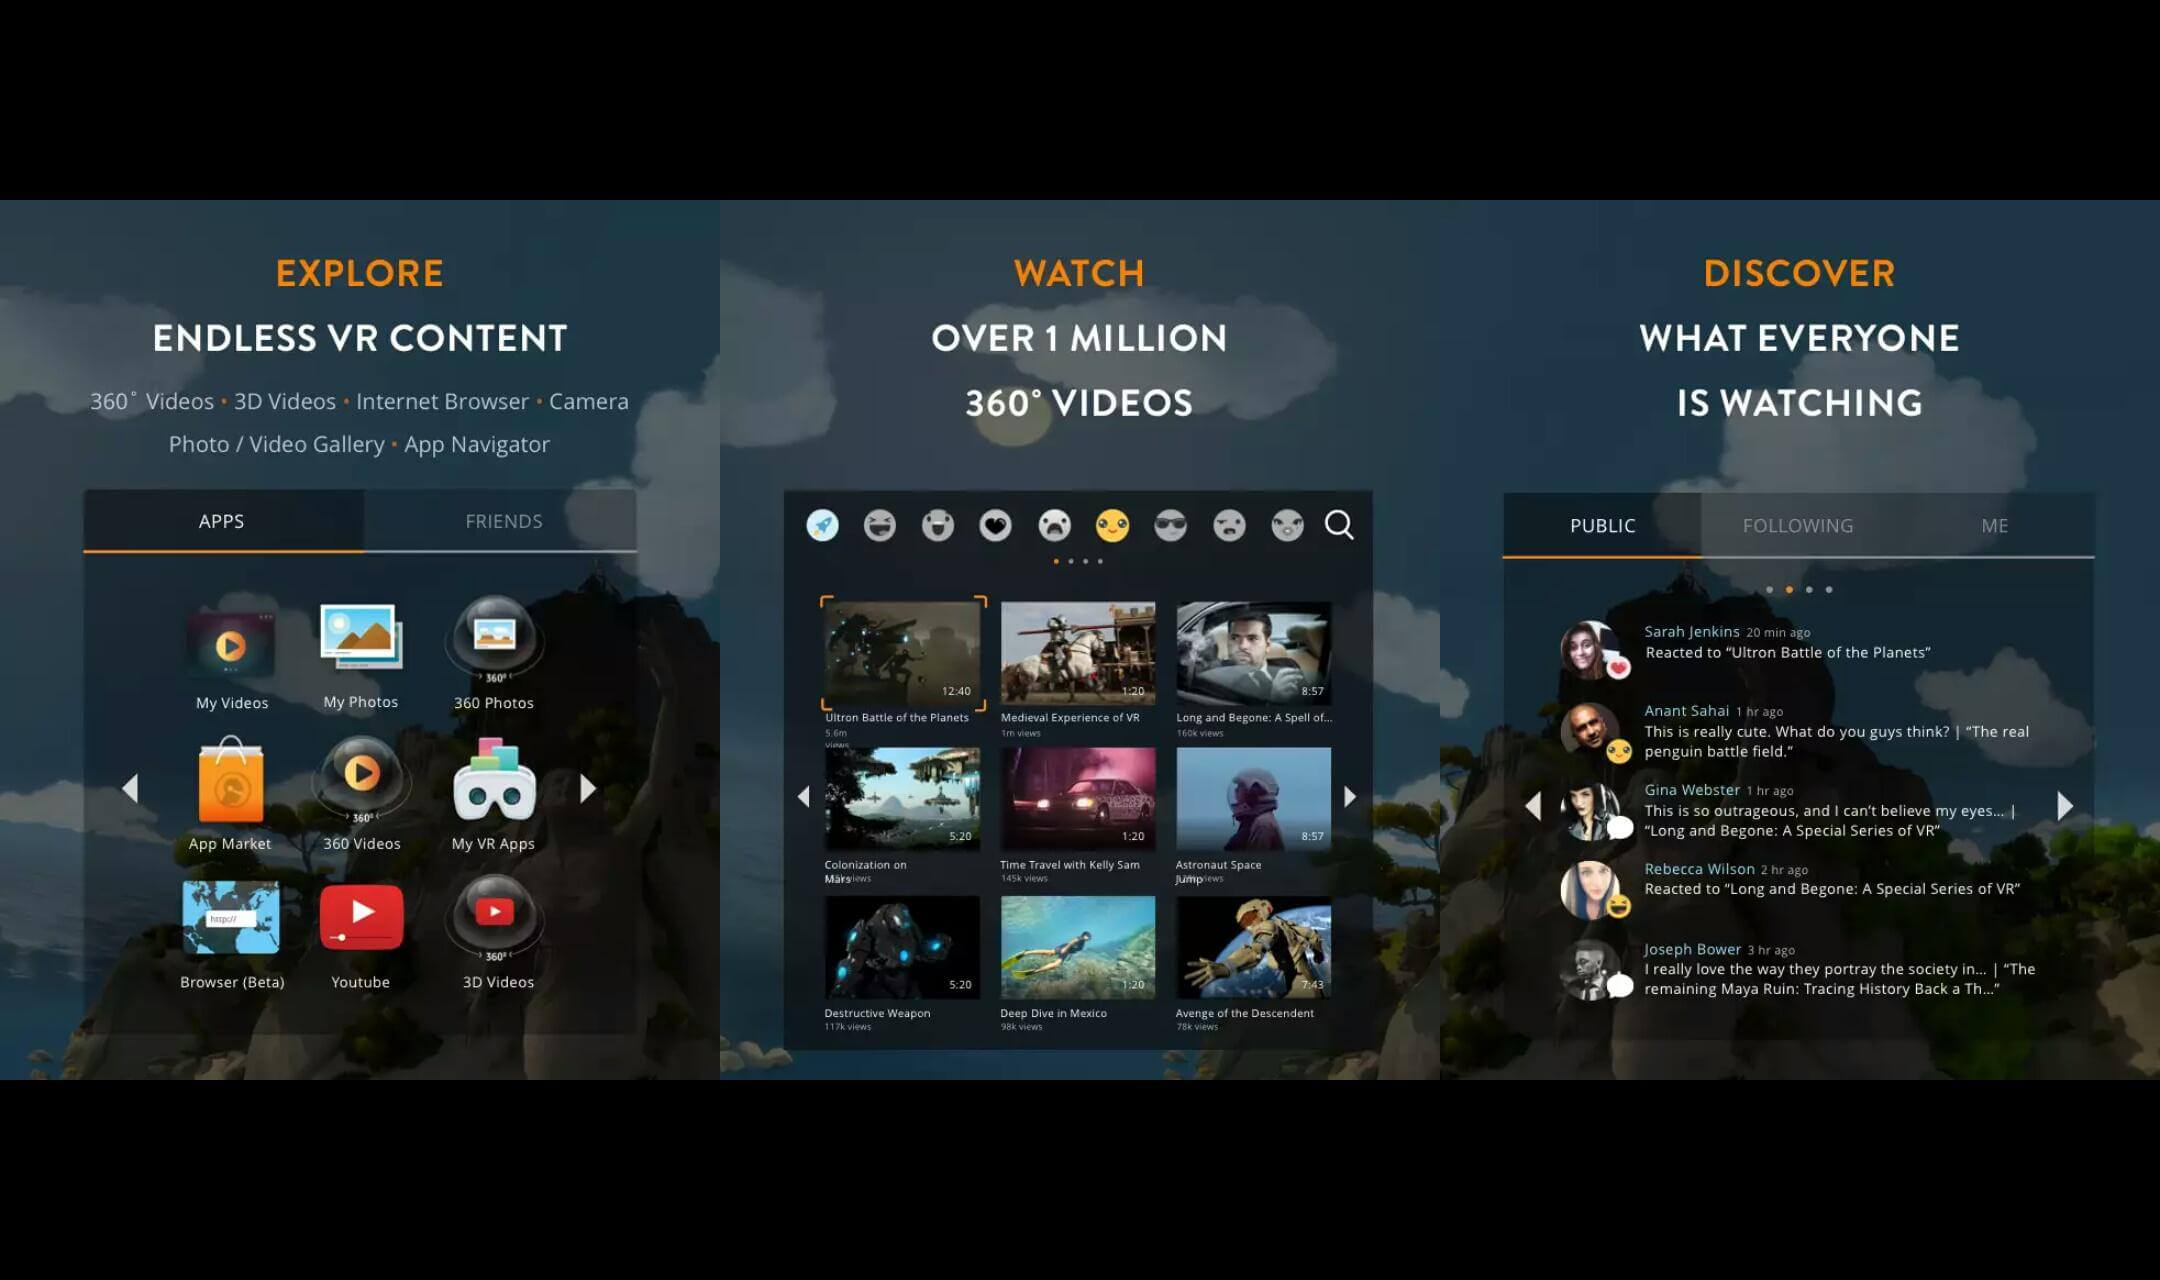
\includegraphics[width=.7\textwidth]{fulldive1}
}
\caption{Fulldive 内置的应用列表}
\label{fig:fulldive1}
\end{figure}

与 Ascape 不同之处在于 Fulldive 的操控完全是在虚拟全景中,所以在播放视频及操作选项时 Fulldive 有一些针对配戴虚拟现实眼镜者所特别提供的操作方式,见图\ref{fig:fulldive2}。例如,将视线聚焦在某个按钮上超过 3 秒后即视为按下了该按钮。这种交互形式借鉴了鼠标的双击或是触屏的长按这两种操作,同时兼顾到视线对齐对人操作的便捷性和可操作性,见图\ref{fig:fulldive3}。

\begin{figure}[htp]
\centering
\fbox{
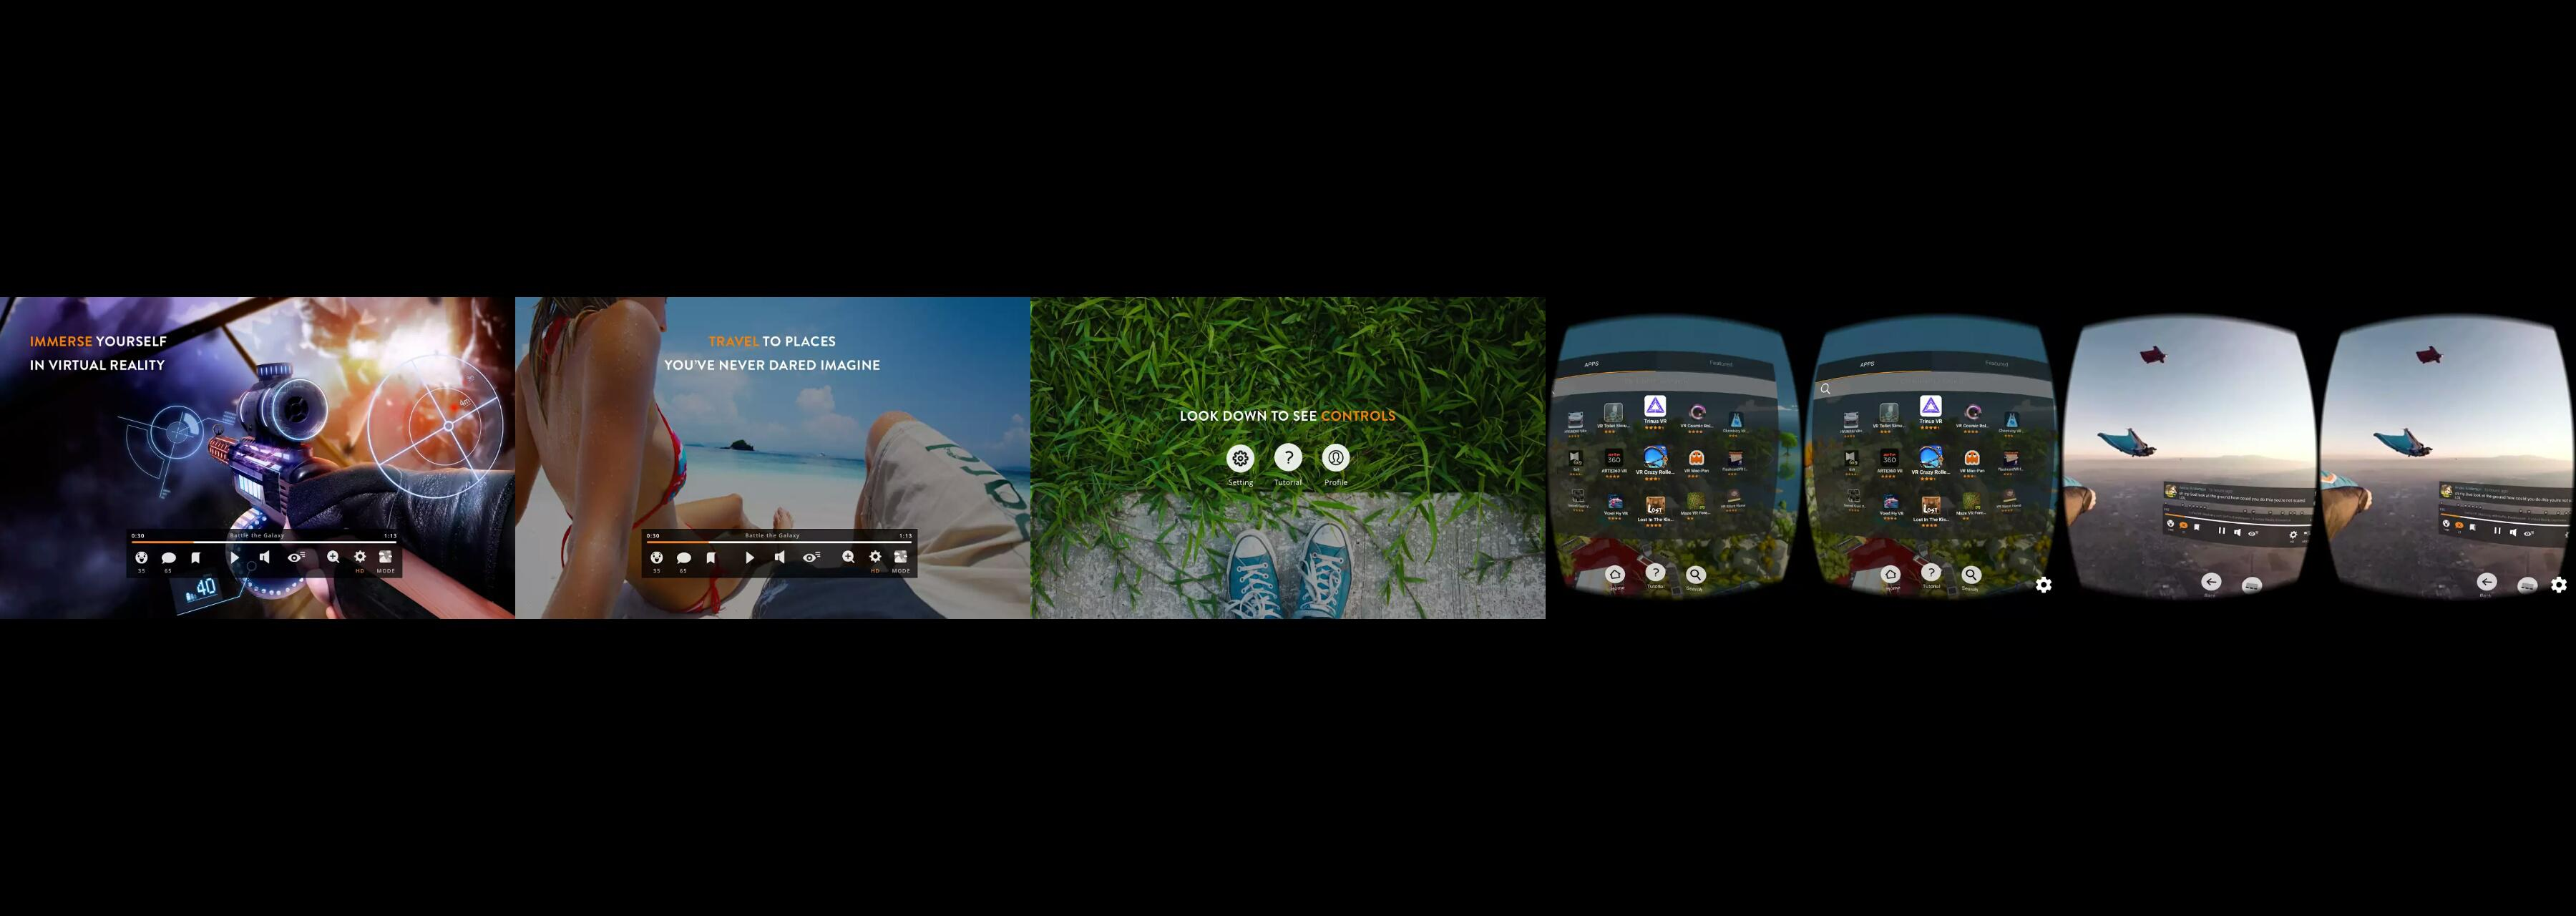
\includegraphics[width=.6\textwidth]{fulldive2}
}
\caption{Fulldive 特有操作形式}
\label{fig:fulldive2}
\end{figure}

\begin{figure}[htp]
\centering
\fbox{
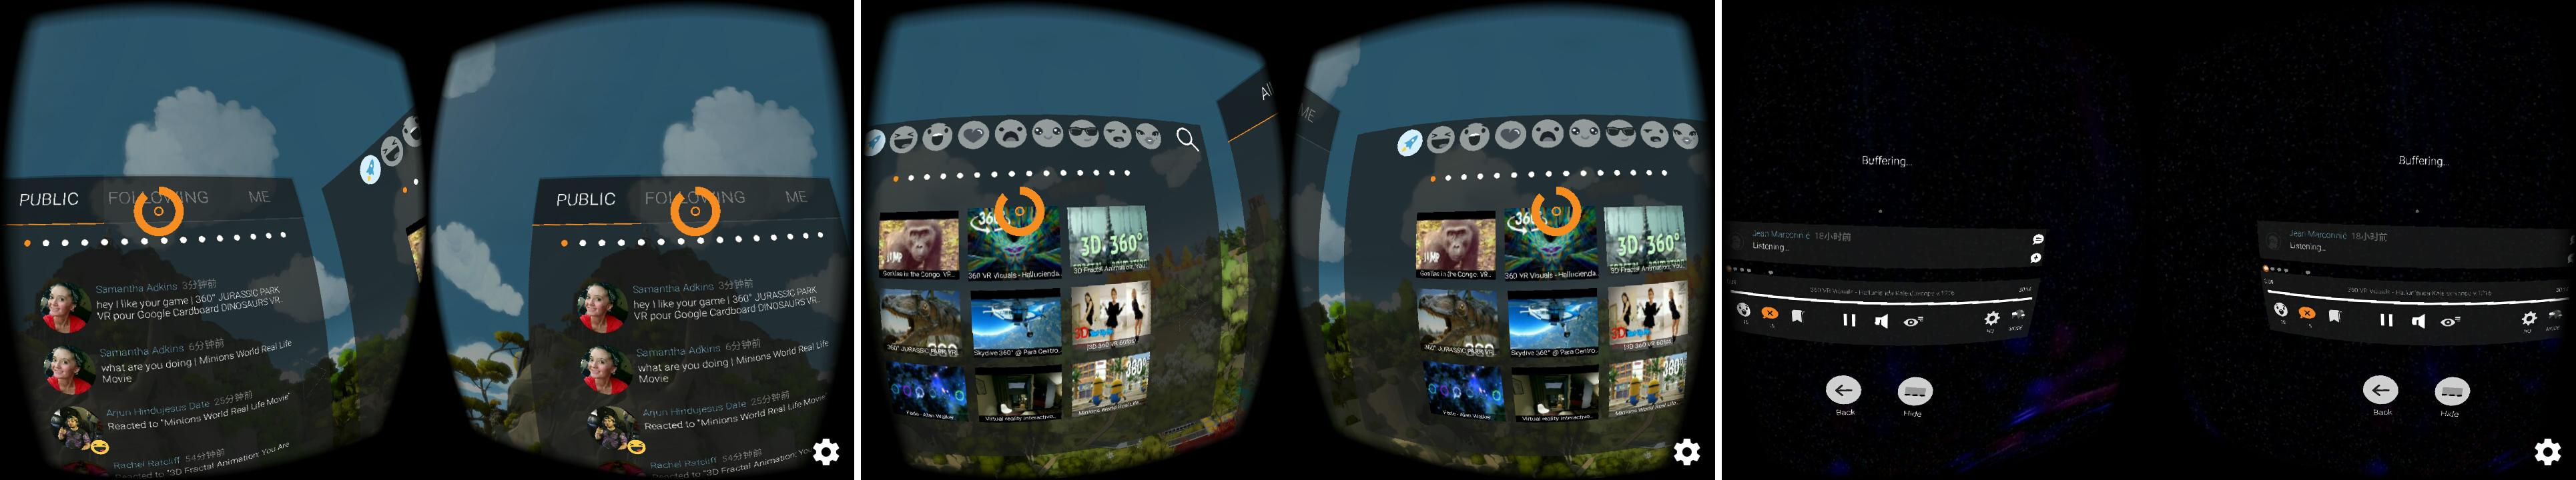
\includegraphics[width=.6\textwidth]{fulldive3}
}
\caption{Fulldive 视线停留模拟点击}
\label{fig:fulldive3}
\end{figure}

当然,这种模拟点击的操作只适用于”确认/取消“这种布尔判断的操作,用户需要输入大段的文字时则需有更高效的方式。Fulldive 结合了已日益成熟的语音识别技术,图\ref{fig:fulldive4}为实际操作 Fulldive 搜索功能并口述”中国地质大学“后的操作截屏。

\begin{figure}[htp]
\centering
\fbox{
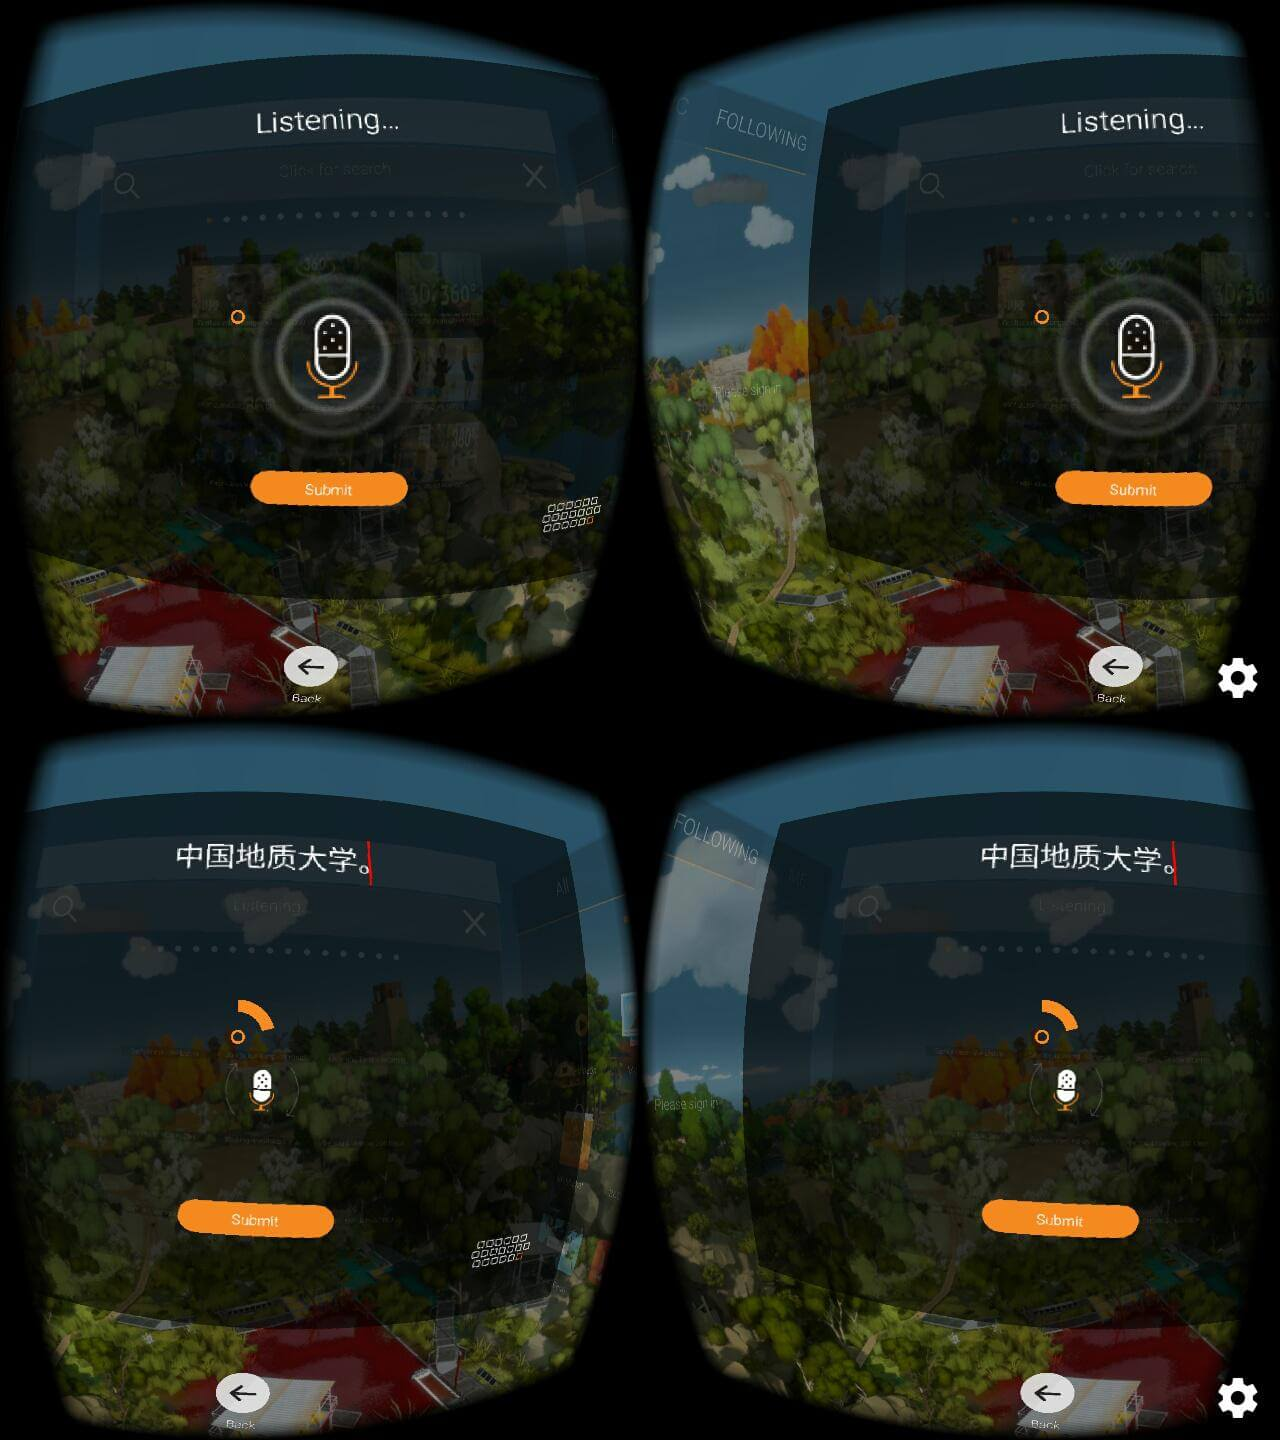
\includegraphics[width=.5\textwidth]{fulldive4}
}
\caption{Fulldive 语音识别}
\label{fig:fulldive4}
\end{figure}

\subsection{VR X-Racer}

VR X-Racer 是一款越南公司于 2016 年开发的简单的 VR 操控类飞行游戏,其操作方式为晃动设备(如 VR 眼镜或手机)来控制屏幕上的飞机躲避障碍物,见图\ref{fig:x-racer}。这是全景漫游技术在游戏上最直接的体现:几乎没有多余的操作,在游戏中飞机撞到障碍物坠毁后无操作若干秒即自动重新游戏。但其最大的缺陷是无法长时间使用,不断晃动的全景屏幕容易使人产生眩晕、恶心等不良反应。
全景漫游与 3D 影片的体验是完全不同的,全景漫游将用户完全包裹在视频所构建的封闭环境中,而 3D 眼镜只是对屏幕这种有限区域进行了折射。两者的区别在于 3D 影片由于有周围环境作为铺垫不易使人完全沉浸其中,全景漫游则是在很短的时间内(20-30 秒)就使人沉浸在虚拟世界中,直至摘掉全景设备重新适应周围环境。

\begin{figure}[htp]
\centering
\fbox{
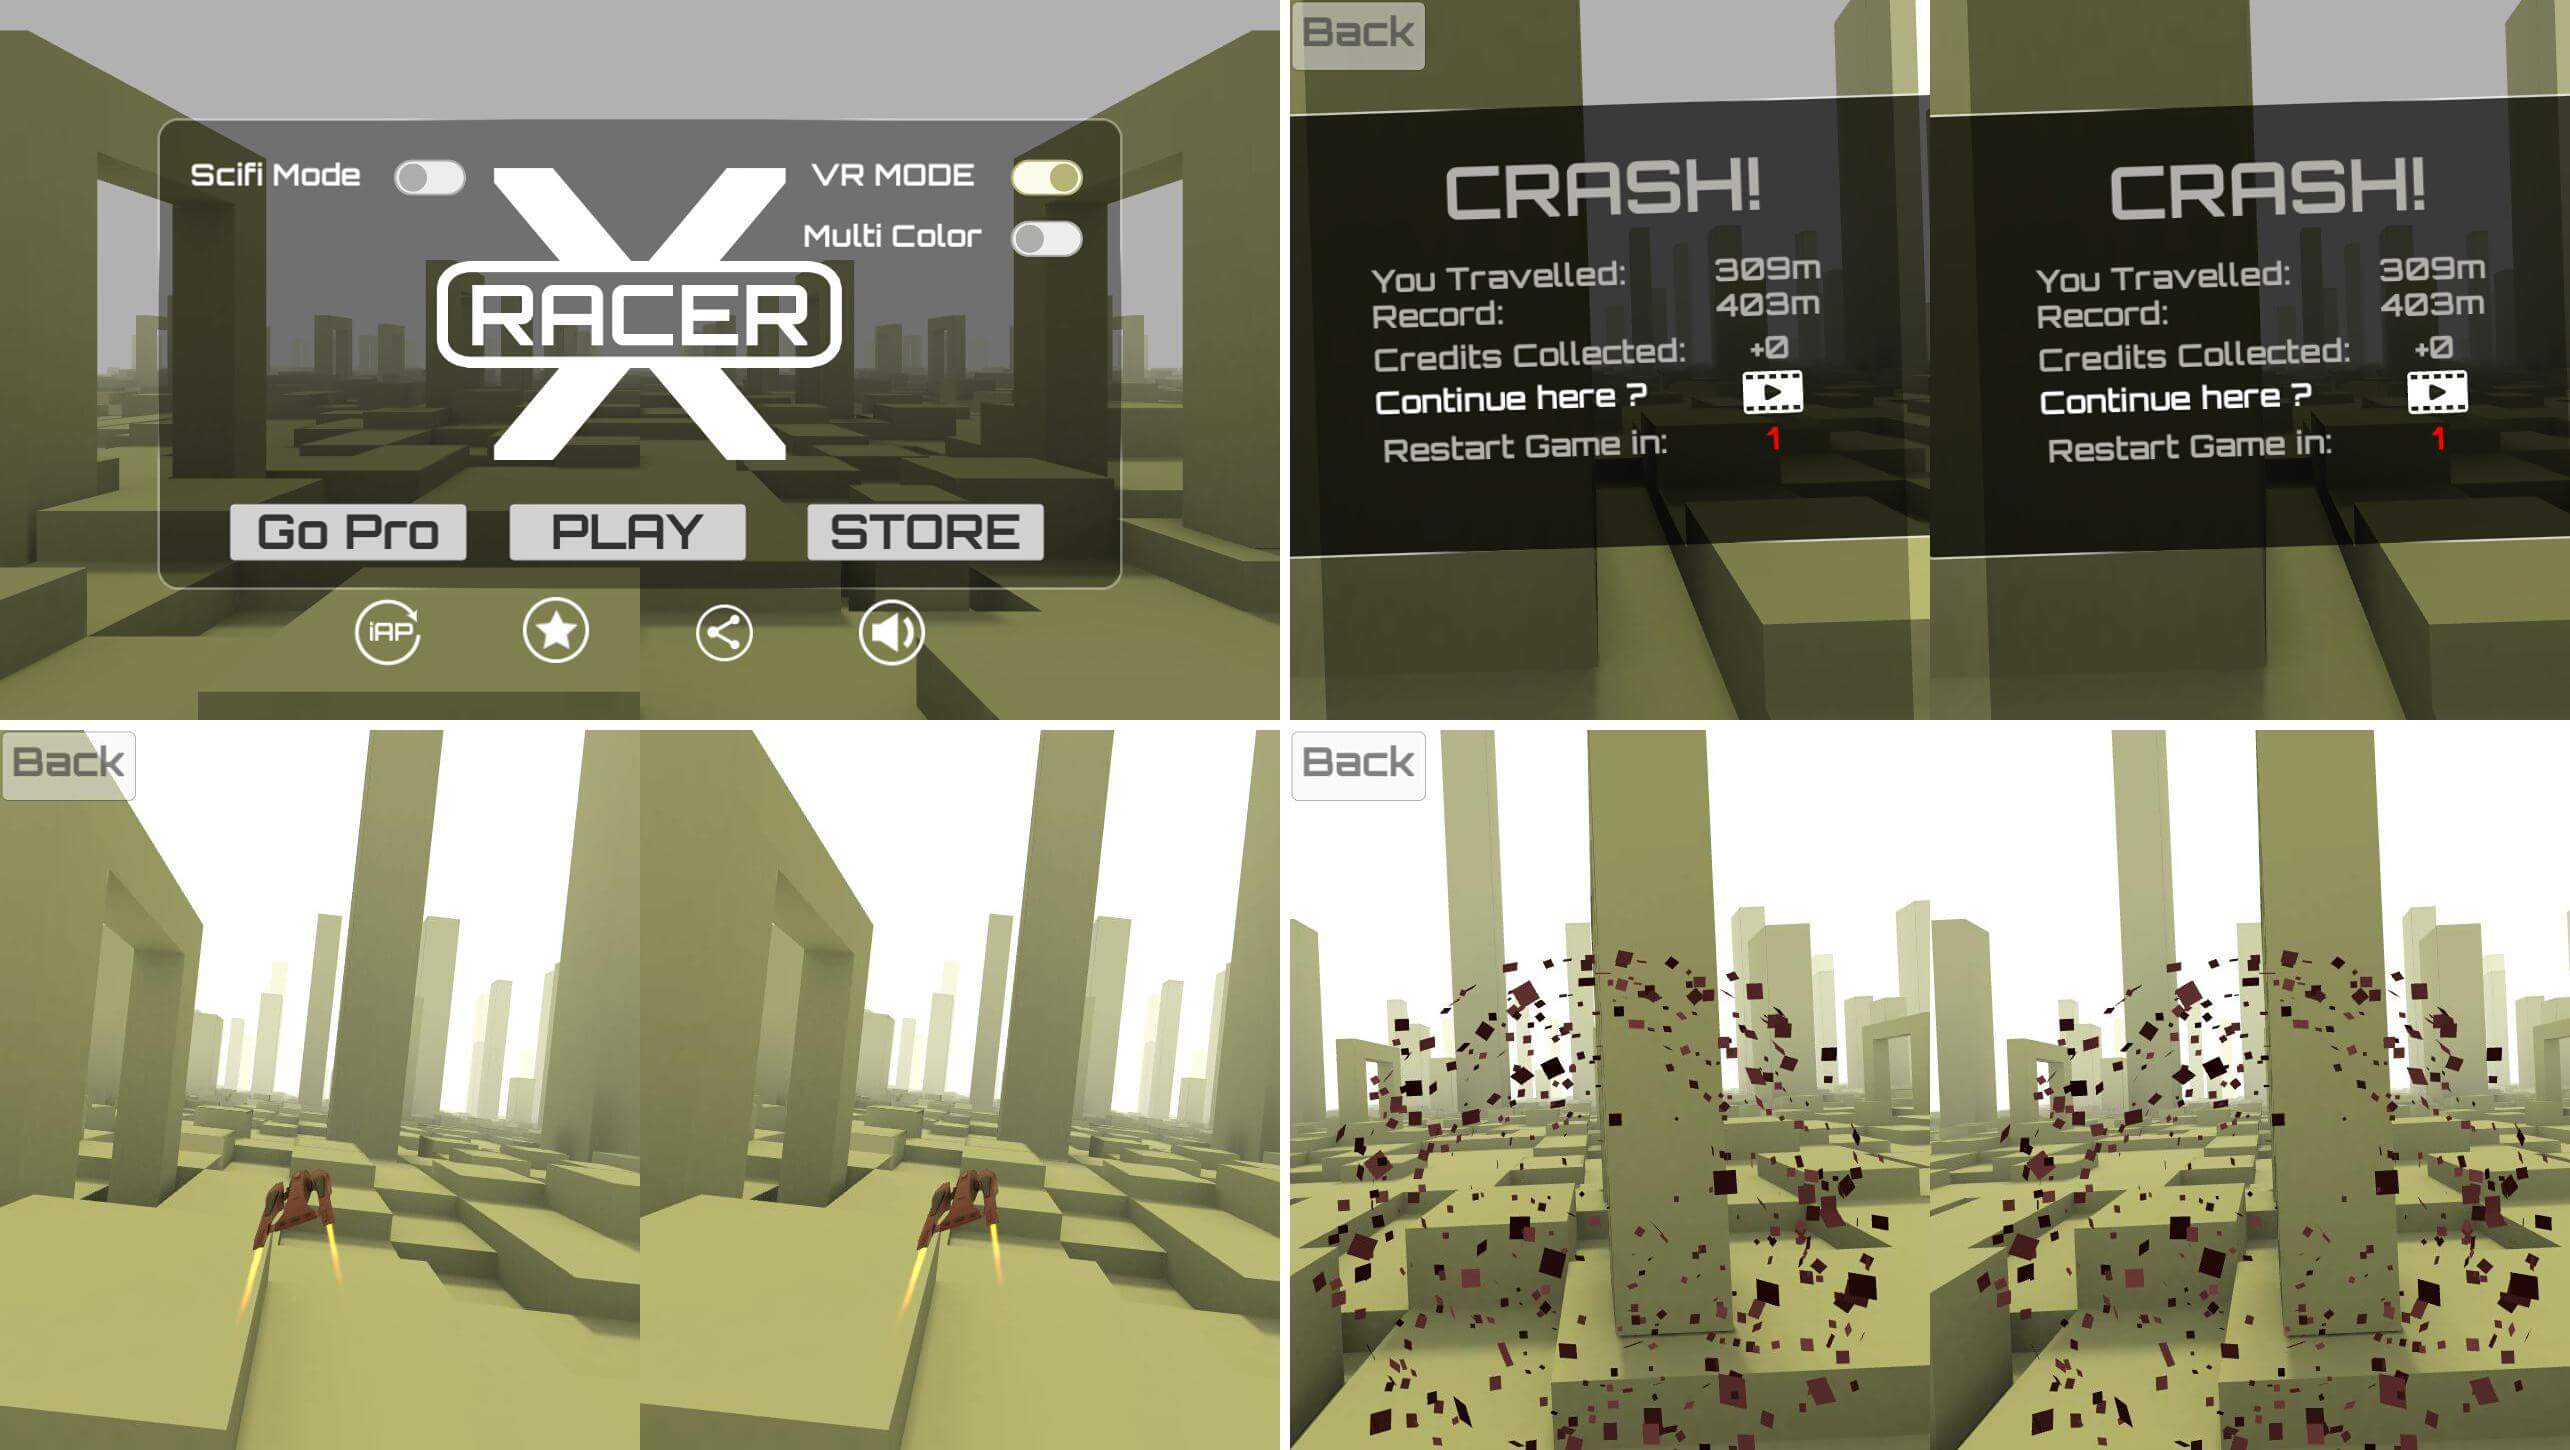
\includegraphics[width=.5\textwidth]{x-racer}
}
\caption{X-racer 游戏截图}
\label{fig:x-racer}
\end{figure}

\subsection{暴风魔镜 VR}

暴风影音是国内在全景漫游生态领域探索前沿的产品之一,最早产品发布于 2014 年,其高端产品售价可达数千元,甚至与国外高端虚拟现实设备如 Oculus 和 GearVR 等价格相齐。与其硬件设备配套的则是一款叫做“暴风魔镜 VR”的手机移动应用。

国内移动应用的发展方向一直是“大而全”,这款应用也不例外。暴风魔镜 VR 力图包括网络/本地视频、影音播放与 VR 移动应用等多种应用,形成自己的 VR 平台体系。该应用不但支持普通的移动应用界面操作模式并且同样支持全景漫游的虚拟现实体验模式。

在交互形式上与上文所列举的 Fulldive 类似,均为视线聚焦停留数秒视为确认,但缺少了语音识别输入大段文字的功能(在页面模式下支持手机输入法输入),如图\ref{fig:storm}。总体使用可满足基本的全景漫游体验,但识别速度较慢或误识别是比较严重的问题。

值得注意的一点是,暴风魔镜 VR 移动应用内场景下方有一个“归位”图标,触发后将会调整屏幕主视域至正对当前屏幕的位置,可类比于传统移动应用的“回到顶部”功能。这个功能很方便地起到了定位自身的作用,让用户不必盲目转动来寻找起始时正对着的界面。


\begin{figure}[htp]
\centering
\fbox{
  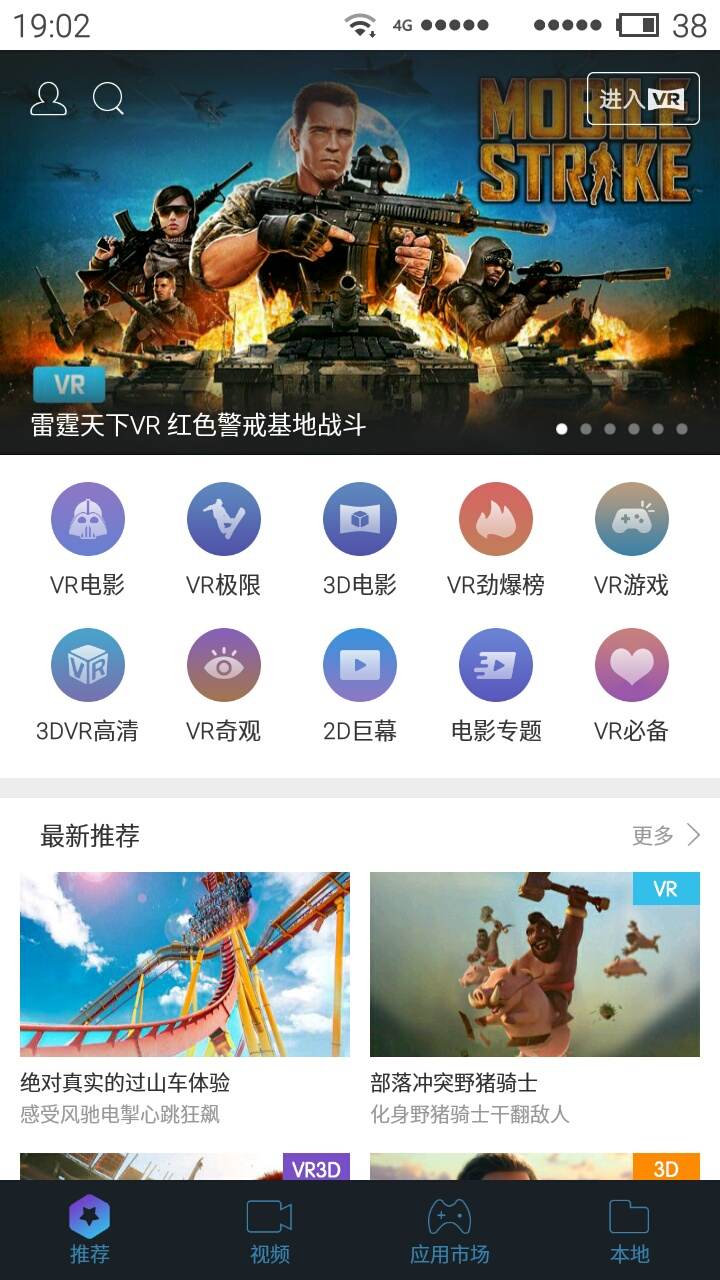
\includegraphics[width=.22\textwidth]{storm1}
}
\fbox{
  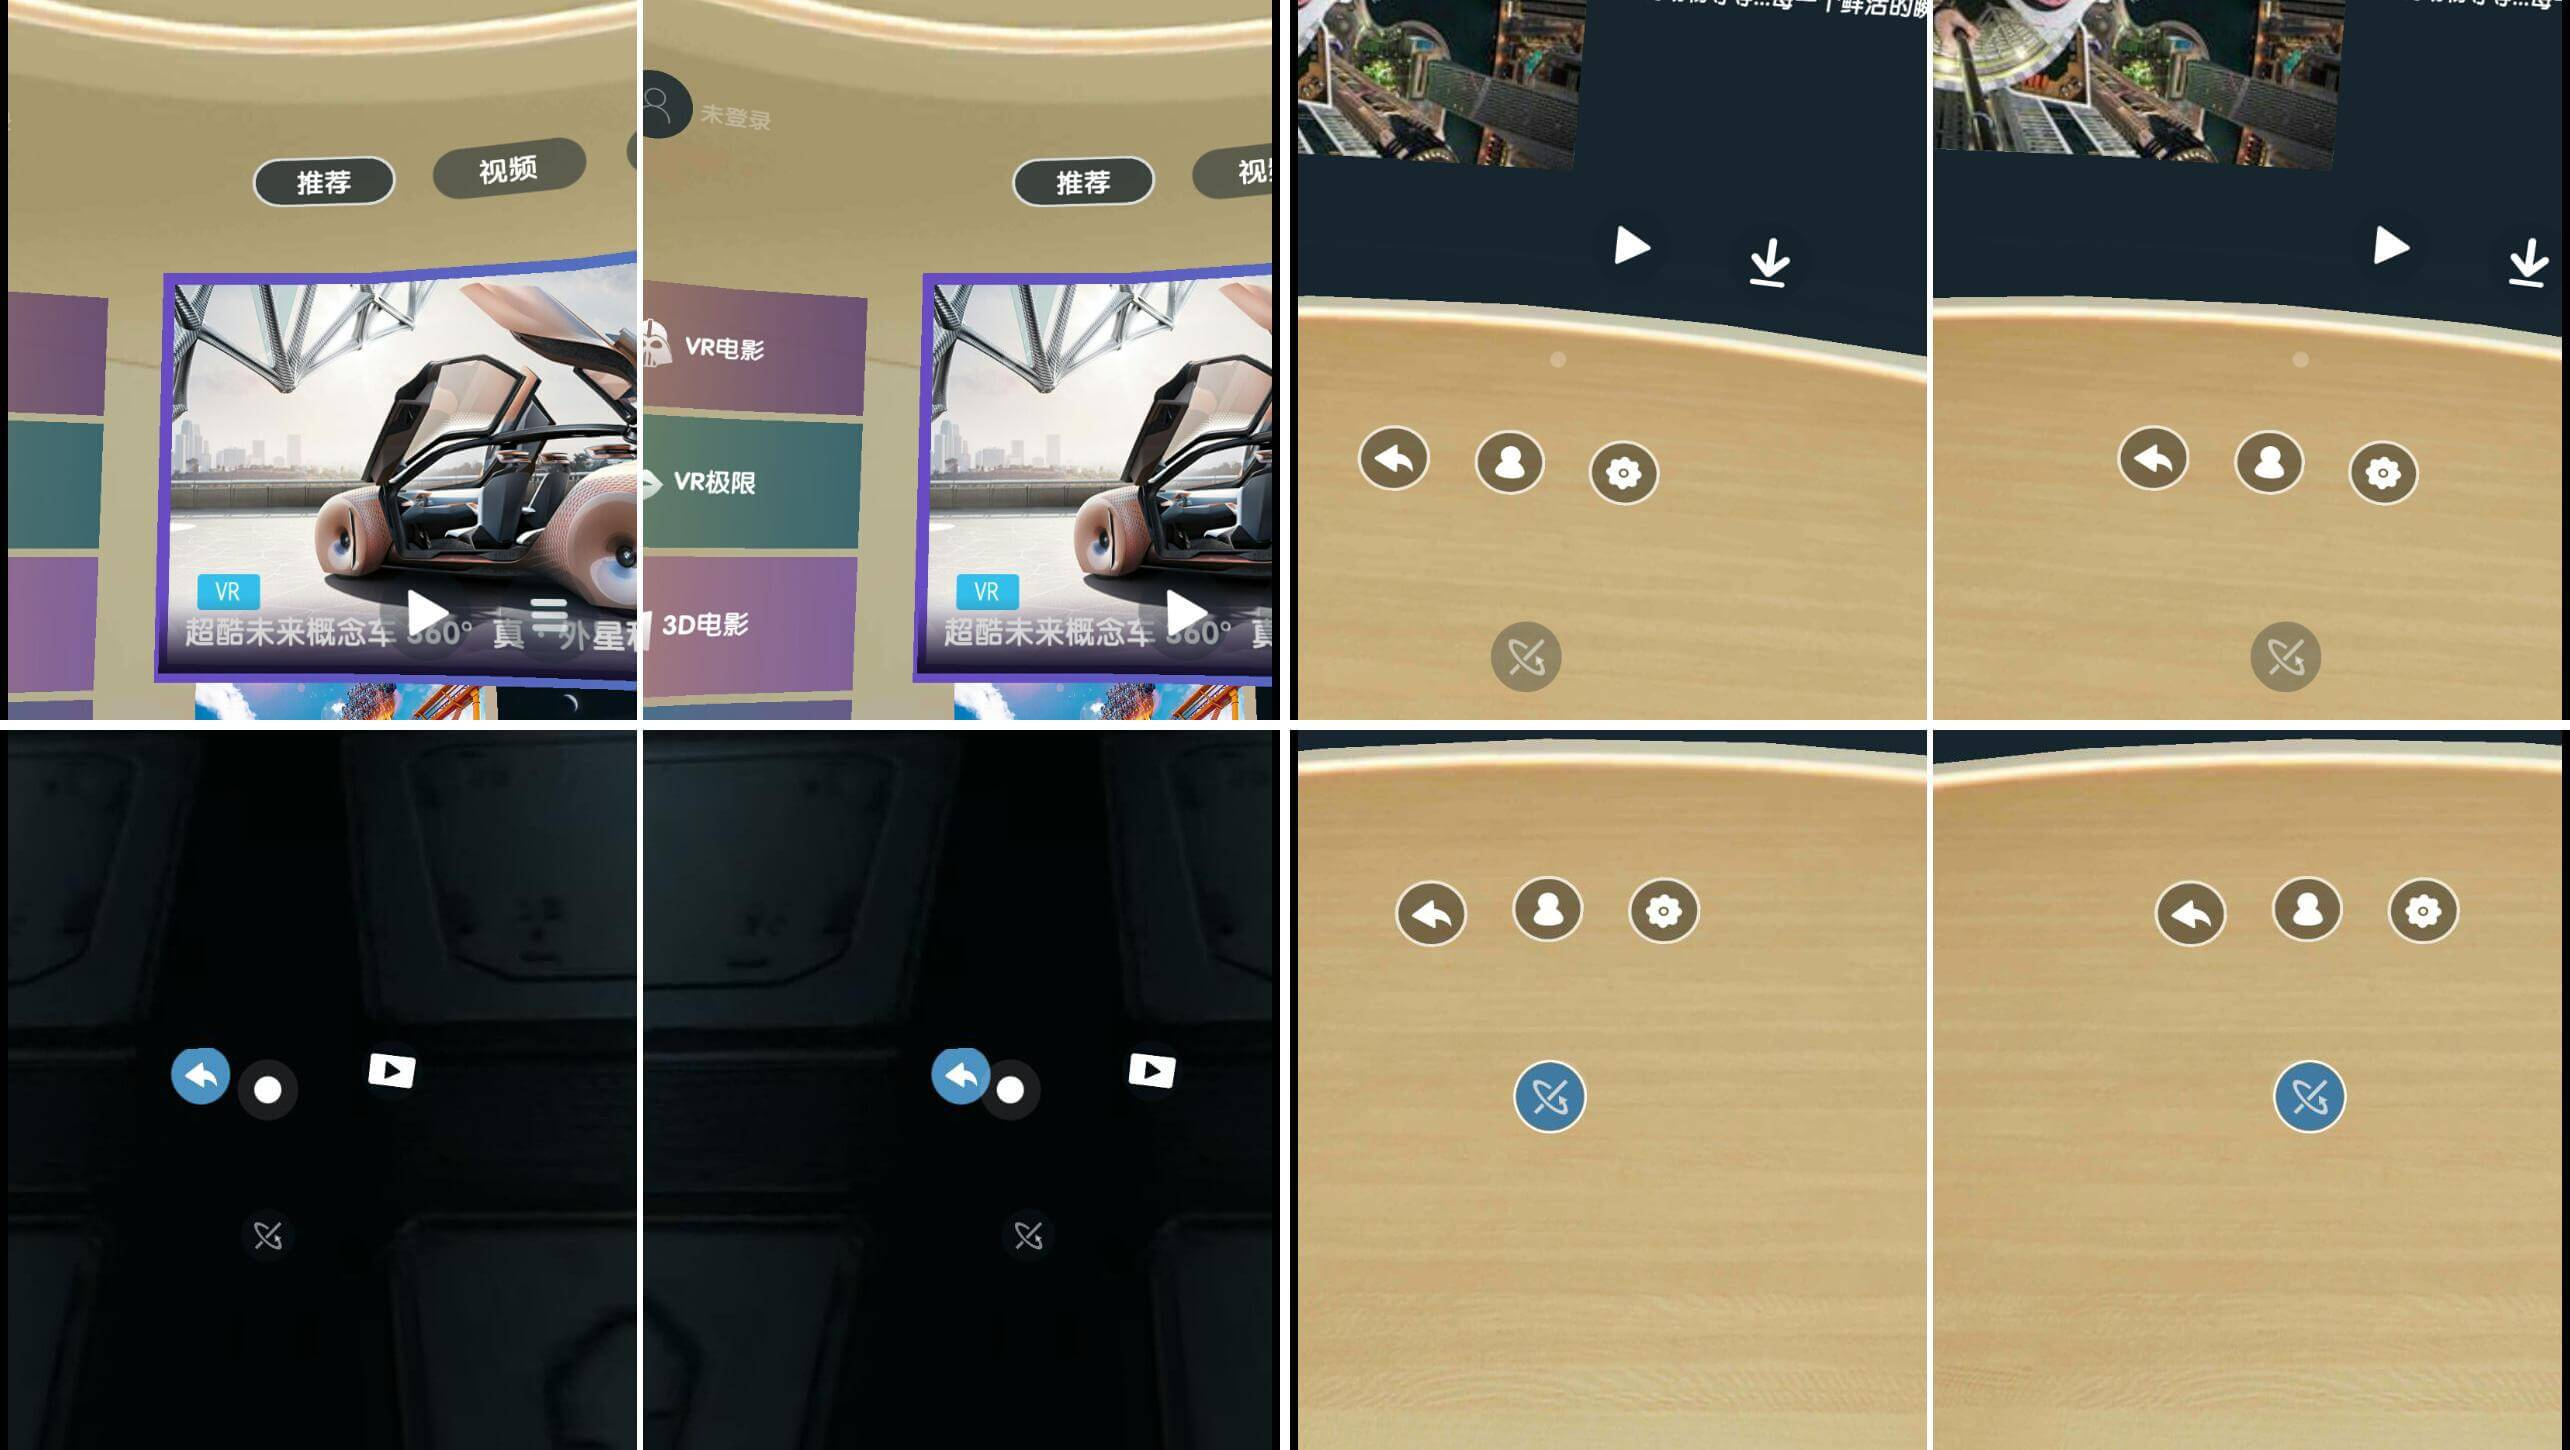
\includegraphics[width=.68\textwidth]{storm2}
}
\caption{暴风魔镜 VR 操作方式}
\label{fig:storm}
\end{figure}

\subsection{国内外移动应用总结}
国外应用较多为单一功能并凸显自身用户体验特色,而国内应用多期望建成平台式产品力图获得更大的市场份额。究其原因,国外此类开发团队小而精,立足于开发特定使用情景和目的的产品,而国内应用常常依附于配套开发的硬件设备,整体呈闭源趋势,故应用局限性较大。国外应用功能较为精简,国内应用则力图提供尽可能多的交互操作形式,但同样在交互层面难以摆脱移动设备平面屏幕所框定的范围。


\section{全景漫游行业现状总结}

全景漫游正处在行业发展的成长期,相关技术发展迅速,但同质化较为严重。众多厂商基于经济利益考量注重硬件设备的研发和更新换代,但软件质量与硬件质量仍有一定的差距,主要体现软件交互设计的质量上。

在全景漫游的交互设计上,国内外 APP 均有较多针对与不同与传统人机界面交互的创新点,例如前文列举的“视线停留数秒确定”、“语音识别”和“底部 Dock 栏”等。但交互可操作性相比于传统人机界面还有一定的差距,例如无法很快定位到所需内容、运动过程中不易操控及场景切换时语境丢失等问题。同时,在全景漫游的现有设计中,仍旧无法脱离面向传统人机界面的设计语境,在考虑保留用户习惯的同时难以创新出更为独特的交互模式,可以说是全景漫游交互设计亟待研究的难点。

全景漫游的行业发展离不开全景漫游的软硬件及生态环境的良好结合,只有如此才能留存有效用户并产生价值,故行业目前的重点就是在软硬件上均体现出应有的价值提升。其中,软件方面可在全景漫游领域的交互方向结合相关理论作出新的设计以改善用户体验。
